\begin{frame}{Backup: per-instance agreement distributions}
\begin{center}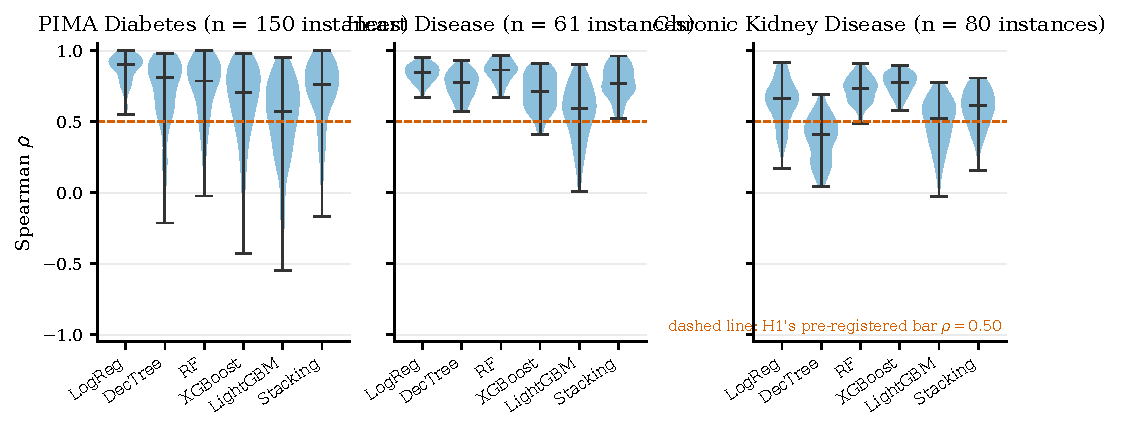
\includegraphics[width=0.95\textwidth]{F5.pdf}\end{center}
\end{frame}

\begin{frame}{Backup: LIME's variance is a budget you choose}
\begin{center}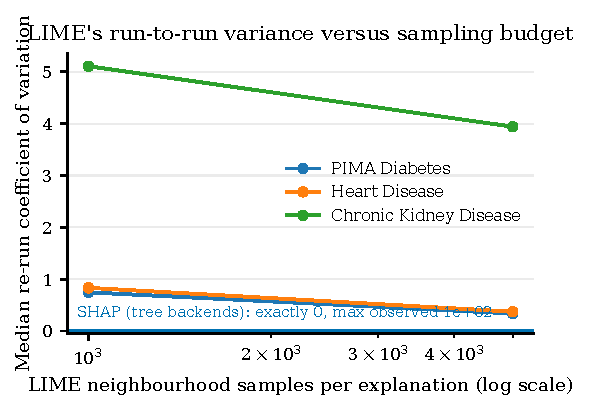
\includegraphics[width=0.62\textwidth]{F7.pdf}\end{center}
\end{frame}

\begin{frame}{Backup: retraining stability, the three ensembles}
\begin{center}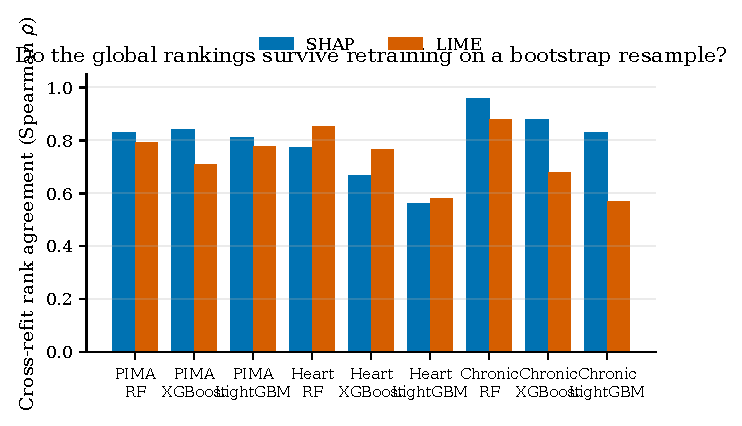
\includegraphics[width=0.78\textwidth]{F9.pdf}\end{center}
\end{frame}

\begin{frame}{Backup: dataset characteristics and missingness}
\begin{center}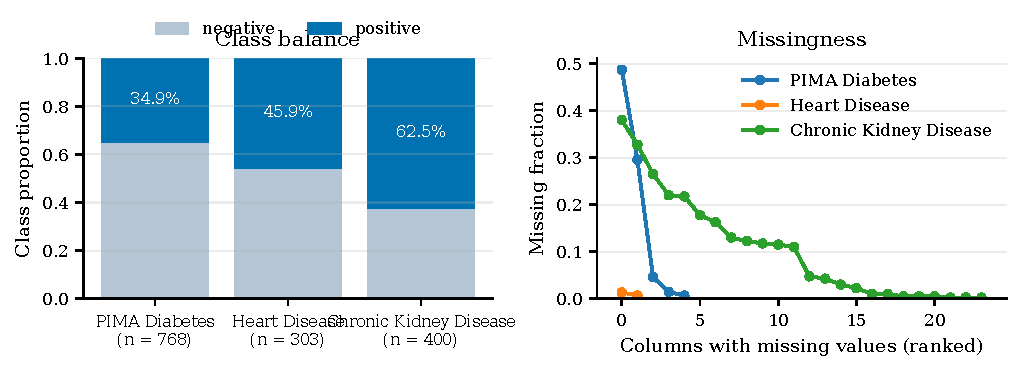
\includegraphics[width=0.95\textwidth]{F2.pdf}\end{center}
\end{frame}

\begin{frame}{Backup: ``What exactly is novel here?''}
\small
Three claims, each verifiable from a named table:
\begin{enumerate}\setlength\itemsep{0.4em}
  \item A \textbf{controlled benchmark} --- \NumCells{} cells, one protocol, 11
    pre-registered hypotheses, Holm-corrected, effect sizes and intervals throughout.
  \item A \textbf{stability decomposition} into three separable sources measured on the
    same models.
  \item A \textbf{hybrid consensus method} --- fidelity-weighted rank fusion --- against
    two published baselines and a strict bar.
\end{enumerate}
\medskip
We claim no priority for explanation aggregation itself --- that is prior work and we
cite it. Ours is the fidelity weighting, the leakage-safe calibration split, and the
controlled test. An evaluation claim cannot be refuted by a citation.
\end{frame}

\begin{frame}{Backup: ``Your SHAP stability result is trivially zero''}
\small
Correct --- and stated in the protocol \emph{before} the experiment ran, because
\textsc{TreeExplainer} is deterministic given a fixed background. Reporting it as a
discovery would be the error.
\medskip
The informative measurements are the other two:
\begin{itemize}
  \item perturbation robustness $\hat L$: \LipschitzShap{} vs \LipschitzLime{} ---
    non-trivial for both
  \item retraining stability: \RetrainShap{} vs \RetrainLime{} --- and this is where a
    deterministic explainer's guarantee runs out
\end{itemize}
The stacking cells are also informative for re-run variance, since they admit no tree
backend and \shap{} is sampling-based there.
\end{frame}

\begin{frame}{Backup: ``Isn't median imputation off-manifold?''}
\small
Yes --- Hooker et al.\ (2019) is exactly this objection, and we do not dispute it.
\medskip
Which is why every fidelity measurement is repeated with baselines drawn from each
feature's observed training marginal, so perturbed rows stay marginally plausible. The
ordering of the explainers did not reverse.
\medskip
Both variants still assume feature independence. A fully on-manifold evaluation needs a
generative model of the data, which we name as future work rather than gesture at.
\end{frame}

\begin{frame}{Backup: ``Did you correct for multiple comparisons?''}
\small
Holm--Bonferroni \emph{within} each hypothesis family --- the family being the set of
cells that hypothesis spans (18 for most, 36 for the control comparisons, 9 for
retraining). Both raw and adjusted $p$ are reported for every test; decisions use the
adjusted value.
\medskip
Degenerate cells --- those with no variation to test, expected for tree \shap{} --- are
kept in the table and reported, but excluded from the correction divisor. Correcting a
test that was never performed only discards power.
\medskip
With hundreds of instances per cell, significance is cheap. The effect size is the
finding, and it appears beside every $p$-value.
\end{frame}

\begin{frame}{Backup: ``Three datasets is not many''}
\small
Agreed, and it is the study's main limitation.
\medskip
The design compensation is the \textbf{difficulty gradient}: ROC-AUC \AucPima{} to
\AucCkd{}, which lets us ask a question a wider but flatter set of datasets could not.
\medskip
On reflection we would widen the dataset axis before the model axis --- four models
across eight datasets would support a stronger claim for the same compute. That is
recorded in the report's ``what we would do differently''.
\end{frame}

\begin{frame}{Backup: how to reproduce}
\small
\begin{itemize}\setlength\itemsep{0.4em}
  \item \texttt{make setup} --- virtualenv from \texttt{requirements.lock.txt}
  \item \texttt{make data} --- download, verify SHA-256, vendor locally
  \item \texttt{make test} --- the full suite, including metric correctness against
    analytically known answers
  \item \texttt{make smoke} --- entire pipeline plus document builds in $\sim$5 minutes
  \item \texttt{make all} --- \textsc{full} run, then paper, report, and slides
\end{itemize}
\medskip
\texttt{results/MANIFEST.json} carries a SHA-256 per artefact, the git commit, the
complete seed set, resolved library versions, and the hardware.
\end{frame}
